\subsection{Save and Load File}
A file existed for a game to record the game situation, and continuous playing of an unfinished game or a customized game can be executed. The file is written as a text by using GSON format to represent the whole game situation, just as the Figure \ref{fig: JSONFile} below. 


\begin{figure}[h]
	\centering
	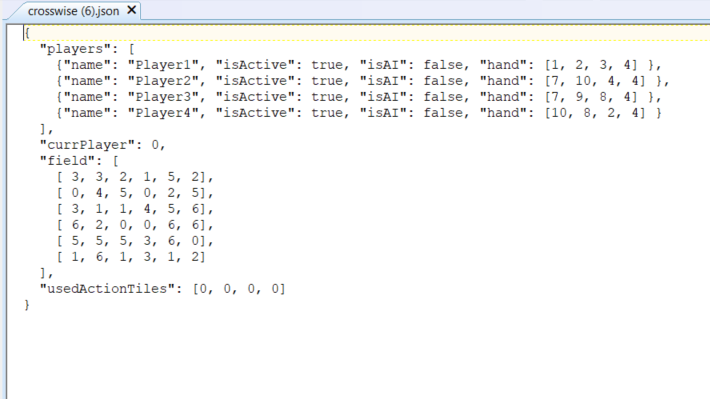
\includegraphics[width=0.8\textwidth]{image/JSON format}
	\caption{The representation of GSON}
	\label{fig: JSONFile}
\end{figure}


\subsubsection{Save}

In the program, the player class could provide the name of the player, active state, AI situation, and the hand token of this player and transfer them into text format.

Additionally, the current player and the field of the whole game board could be transformed into a number representation. Although the board tokens are presented as an enum element, in the board class, we create a method that can be transforming that enum element into an int representation. 

At last, this archive also must involve the list of the used action token, which can remind players of the amount remained number of the action token. The list of action tokens has already used the int array to track in the logic class.

Those transferring behaviors would need to use the getter methods of the class GraphDataJson to complete. 

The ultimate text representation is shown as Figure \ref{fig: JSONFile}.


\subsubsection{Load}

Likewise, loading a game with an archive, in which the file format is as the Figure \ref{fig: JSONFile}. And the recorded attributes must be bound with the attribute in the program.  With the purpose of assigning the value to the program attribute, the setter method of the class GraphDataJson could be used to set up. 